\documentclass[]{article}
\usepackage{lmodern}
\usepackage{amssymb,amsmath}
\usepackage{ifxetex,ifluatex}
\usepackage{fixltx2e} % provides \textsubscript
\ifnum 0\ifxetex 1\fi\ifluatex 1\fi=0 % if pdftex
  \usepackage[T1]{fontenc}
  \usepackage[utf8]{inputenc}
\else % if luatex or xelatex
  \ifxetex
    \usepackage{mathspec}
  \else
    \usepackage{fontspec}
  \fi
  \defaultfontfeatures{Ligatures=TeX,Scale=MatchLowercase}
\fi
% use upquote if available, for straight quotes in verbatim environments
\IfFileExists{upquote.sty}{\usepackage{upquote}}{}
% use microtype if available
\IfFileExists{microtype.sty}{%
\usepackage{microtype}
\UseMicrotypeSet[protrusion]{basicmath} % disable protrusion for tt fonts
}{}
\usepackage[margin=1in]{geometry}
\usepackage{hyperref}
\hypersetup{unicode=true,
            pdftitle={Statistical Power, Statistical Significance, Study Design and Decision Making: A Worked Example},
            pdfauthor={Ben Anderson and Tom Rushby (Contact: b.anderson@soton.ac.uk, @dataknut)},
            pdfborder={0 0 0},
            breaklinks=true}
\urlstyle{same}  % don't use monospace font for urls
\usepackage{longtable,booktabs}
\usepackage{graphicx,grffile}
\makeatletter
\def\maxwidth{\ifdim\Gin@nat@width>\linewidth\linewidth\else\Gin@nat@width\fi}
\def\maxheight{\ifdim\Gin@nat@height>\textheight\textheight\else\Gin@nat@height\fi}
\makeatother
% Scale images if necessary, so that they will not overflow the page
% margins by default, and it is still possible to overwrite the defaults
% using explicit options in \includegraphics[width, height, ...]{}
\setkeys{Gin}{width=\maxwidth,height=\maxheight,keepaspectratio}
\IfFileExists{parskip.sty}{%
\usepackage{parskip}
}{% else
\setlength{\parindent}{0pt}
\setlength{\parskip}{6pt plus 2pt minus 1pt}
}
\setlength{\emergencystretch}{3em}  % prevent overfull lines
\providecommand{\tightlist}{%
  \setlength{\itemsep}{0pt}\setlength{\parskip}{0pt}}
\setcounter{secnumdepth}{5}
% Redefines (sub)paragraphs to behave more like sections
\ifx\paragraph\undefined\else
\let\oldparagraph\paragraph
\renewcommand{\paragraph}[1]{\oldparagraph{#1}\mbox{}}
\fi
\ifx\subparagraph\undefined\else
\let\oldsubparagraph\subparagraph
\renewcommand{\subparagraph}[1]{\oldsubparagraph{#1}\mbox{}}
\fi

%%% Use protect on footnotes to avoid problems with footnotes in titles
\let\rmarkdownfootnote\footnote%
\def\footnote{\protect\rmarkdownfootnote}

%%% Change title format to be more compact
\usepackage{titling}

% Create subtitle command for use in maketitle
\newcommand{\subtitle}[1]{
  \posttitle{
    \begin{center}\large#1\end{center}
    }
}

\setlength{\droptitle}{-2em}

  \title{Statistical Power, Statistical Significance, Study Design and Decision
Making: A Worked Example}
    \pretitle{\vspace{\droptitle}\centering\huge}
  \posttitle{\par}
  \subtitle{Sizing Demand Response Trials in New Zealand}
  \author{Ben Anderson and Tom Rushby (Contact:
\href{mailto:b.anderson@soton.ac.uk}{\nolinkurl{b.anderson@soton.ac.uk}},
\texttt{@dataknut})}
    \preauthor{\centering\large\emph}
  \postauthor{\par}
      \predate{\centering\large\emph}
  \postdate{\par}
    \date{Last run at: 2018-09-18 18:04:39}

\usepackage{booktabs}
\usepackage{longtable}
\usepackage{array}
\usepackage{multirow}
\usepackage[table]{xcolor}
\usepackage{wrapfig}
\usepackage{float}
\usepackage{colortbl}
\usepackage{pdflscape}
\usepackage{tabu}
\usepackage{threeparttable}
\usepackage{threeparttablex}
\usepackage[normalem]{ulem}
\usepackage{makecell}

\usepackage{amsthm}
\newtheorem{theorem}{Theorem}[section]
\newtheorem{lemma}{Lemma}[section]
\theoremstyle{definition}
\newtheorem{definition}{Definition}[section]
\newtheorem{corollary}{Corollary}[section]
\newtheorem{proposition}{Proposition}[section]
\theoremstyle{definition}
\newtheorem{example}{Example}[section]
\theoremstyle{definition}
\newtheorem{exercise}{Exercise}[section]
\theoremstyle{remark}
\newtheorem*{remark}{Remark}
\newtheorem*{solution}{Solution}
\begin{document}
\maketitle

{
\setcounter{tocdepth}{2}
\tableofcontents
}
\newpage

\section{About}\label{about}

\subsection{Report circulation:}\label{report-circulation}

\begin{itemize}
\tightlist
\item
  Public
\end{itemize}

\subsection{License}\label{license}

\subsection{Citation}\label{citation}

If you wish to use any of the material from this report please cite as:

\begin{itemize}
\tightlist
\item
  Ben Anderson and Tom Rushby. (2018) Statistical Power, Statistical
  Significance, Study Design and Decision Making: A Worked Example
  (Sizing Demand Response Trials in New Zealand),
  \href{http://www.otago.ac.nz/centre-sustainability/}{Centre for
  Sustainability}, University of Otago: Dunedin, New Zealand.
\end{itemize}

This work is (c) 2018 the authors.

\subsection{History}\label{history}

Code history is generally tracked via our git.soton
\href{https://github.com/CfSOtago/GREENGrid}{repo}:

\begin{itemize}
\tightlist
\item
  \href{https://github.com/CfSOtago/GREENGrid/commits/master/analysis/powerAnalysis}{Report
  history}
\end{itemize}

\subsection{Data:}\label{data}

This paper uses circuit level extracts for `Heat Pumps', `Lighting' and
`Hot Water' for the NZ GREEN Grid Household Electricity Demand Data
(\url{https://dx.doi.org/10.5255/UKDA-SN-853334} (Anderson et al.
2018)). These have been extracted using the code found in

\subsection{Support}\label{support}

This work was supported by:

\begin{itemize}
\tightlist
\item
  The \href{https://www.otago.ac.nz/}{University of Otago};
\item
  The \href{https://www.southampton.ac.uk/}{University of Southampton};
\item
  The New Zealand \href{http://www.mbie.govt.nz/}{Ministry of Business,
  Innovation and Employment (MBIE)} through the
  \href{https://www.otago.ac.nz/centre-sustainability/research/energy/otago050285.html}{NZ
  GREEN Grid} project;
\item
  \href{http://www.energy.soton.ac.uk/tag/spatialec/}{SPATIALEC} - a
  \href{http://ec.europa.eu/research/mariecurieactions/about-msca/actions/if/index_en.htm}{Marie
  Skłodowska-Curie Global Fellowship} based at the University of Otago's
  \href{http://www.otago.ac.nz/centre-sustainability/staff/otago673896.html}{Centre
  for Sustainability} (2017-2019) \& the University of Southampton's
  Sustainable Energy Research Group (2019-2020).
\end{itemize}

We do not `support' the code but if you notice a problem please check
the \href{https://github.com/CfSOtago/GREENGrid/issues}{issues} on our
\href{https://github.com/CfSOtago/GREENGrid}{repo} and if it doesn't
already exist, please open a new one.

\newpage

\section{Introduction}\label{introduction}

In our experiennce of designing and running empirical studies, whether
experimental or naturalistic, there is ongoing confusion over the
meaning and role of two key statistical terms:

\begin{itemize}
\tightlist
\item
  statistical power
\item
  statistical significance
\end{itemize}

We have found this to be the case both in academic research where the
objective is to establish `the most likely explanation' under academic
conventions and in applied research where the objective is to `make a
robust decision' based on the balance of evidence and probability.

In this brief paper we respond to these confusions using a worked
example: the design of a hypothetical household electricity demand
response trial in New Zealand which seeks to shift the use of Heat Pumps
out of the evening winter peak demand period. We use this example to
explain and demonstrate the role of statistical signficance in testing
for differences and of both statistical signficance and statistical
power in sample design and decision making.

\section{Error, power, significance and decision
making}\label{error-power-significance-and-decision-making}

Two types of error are of concern in both purely academic and applied
research studies:

\begin{itemize}
\tightlist
\item
  Type I: a false positive - an effect is inferred when in fact there is
  none. From a commercial or policy perspective this could lead to the
  implementation of a costly intervention which would be unlikely to
  have the effect expected;
\item
  Type II: a false negative - an effect is not inferred when in fact
  there is one. From a commercial or policy perspective this could lead
  to inaction when an intervention would have been likely to have the
  effect expected.
\end{itemize}

The significance level (p value) of the statistical test to be used
represents the extent to which the observed data matches the null model
to be tested (Wasserstein and Lazar 2016). In most trials the null model
will be a measure of `no difference' between control and intervenion
groups. By convention, the p value \emph{threshold} for rejecting the
null model (the risk of a Type I error) is generally set to 0.05 (5\%)
although this choice is entirely subjective. In commercial or policy
terms an action taken on a larger p value (e.g.~setting the p value
threshold to 10\%) would increase the risk of making a Type I error and
thus implementing a potentially costly intervention that is unlikely to
have the effect desired. However, as we discuss in more detail below,
this is not necessarily \emph{bad practice} as it may reflect the
potential magnitude of an effect, the decision-maker's tolerance of Type
I error risk and the urgency of action.

Statistical power is normally set to 0.8 (80\%) by convention and
represents the pre-study risk of making a Type II error (Greenland et
al. 2016). From a commercial or policy perspective reducing power
(e.g.~to 0.7 or 70\%) will therefore increase the risk of taking no
action when in fact the intervention would probably have had the effect
desired. Statistical power calculations enable the investigator to
estimate the sample size that would be needed to robustly detect an
experimental effect with a given risk of a false positive (Type I error)
or false negative (Type II error) result. This prevents a study from
recruiting too few participants to be able to robustly detect the
hypothesised intervention effect (Delmas, Fischlein, and Asensio 2013)
or wasting resources by recruiting a larger sample than needed.

Previous work has suggested that sample sizes in most energy efficiency
studies may be too low to provide adequate power and so statistically
robust conclusions cannot be drawn at conventional thresholds (Frederiks
et al. 2016) while a more recent review focusing on demand response
studies reaching a similar conclusion (Srivastava, Van Passel, and Laes
2018). It is therefore hardly surprising that a number of studies report
effect sizes which are not statistically significant at conventional
thresholds (Srivastava, Van Passel, and Laes 2018), choose to use lower
statistical significance thresholds (Institute 2006, AECOM (2011), CER
(2012), Schofield et al. (2015)) or both lower statistical power values
\emph{and} statistical significance thresholds (UKPN 2017,UKPN (2018)).

However it would be wrong to conclude that this is \emph{necessarily}
bad practice. Recent discussions of the role of p values in inference
(Greenland et al. 2016, Wasserstein and Lazar (2016)) should remind us
that decisions should never be based only on statistical significance
thresholds set purely by convention. Rather, inference and thus decision
making should be based on:

\begin{itemize}
\tightlist
\item
  statistic effect size - is it 2\% or 22\% (i.e.~is the result
  \emph{important} or \emph{useful}, what is the \emph{bang for buck}?)
\item
  statistic confidence intervals - (i.e.~is there \emph{uncertainty} or
  \emph{variation} in response?)
\item
  statistic p values - (i.e.~what is the risk of a Type I error /
  \emph{false positive})
\end{itemize}

As an example, consider the a study which collected electricity power
demand data for two different groups of households. The data shows that
the mean W for group 1 was 35.14 and for group 2 was 162.67. This is a
(very) large difference in the mean of 127.53.

A t-test of the difference between the groups produces the result shown
below.

\begin{verbatim}
## 
##  Welch Two Sample t-test
## 
## data:  testDT[group == "S"]$meanW and testDT[group == "W"]$meanW
## t = -1.9907, df = 31.47, p-value = 0.05526
## alternative hypothesis: true difference in means is not equal to 0
## 95 percent confidence interval:
##  -258.110005    3.050644
## sample estimates:
## mean of x mean of y 
##  35.13947 162.66915
\end{verbatim}

In this case we have:

\begin{itemize}
\tightlist
\item
  effect size = 127.5296803W or 78.4\% representing a \emph{substantial
  bang for buck} for whatever caused the difference;
\item
  95\% confidence interval for the test = -258.11 to 3.05 representing
  \emph{considerable} uncertainty/variation;
\item
  p value of 0.055 representing a \emph{relatively low} risk of a false
  positive results but which (just) fails the conventional p \textless{}
  0.05 threshold.
\end{itemize}

What would we have concluded? We have a large effect size, substantial
uncertainty and a slightly raised risk of a false positive or Type I
error when compared to conventional p value levels. From a narrow and
conventional `p value testing' perspective we would have concluded that
there was no statistically signficant difference between the groups.
However this misses the crucial point that an organisation with a higher
risk tolerance might conclude that the large effect size justifies
implementing the intervention even though the risk of a false positive
is slightly higher. If the p value had been 0.25 then this would have
still been the case but would have warranted even further caution. As
the recent discussions of the role of the p value in decision making
have made clear (Wasserstein and Lazar 2016) statistical analysis needs
to report all of these elements to enable contextually appropriate and
defensible evidence-based decisions to be taken. Simply dismissing
results on the basis of failure to meet conventional statistical levels
of significance risks throwing both the baby and the bath water out of
the window.

In the following sections we apply these principles to the design and
analysis of a hypothetical New Zealand household electricity demand
response trial.

\section{Sample design: statistical
power}\label{sample-design-statistical-power}

To return to the discussion of statistical power, we need to establish
the probably size of the control and intervention groups we will
require. This is an aid to resource budgeting (\emph{``How many
households and thus \texttt{\$} do I need?''}) and to ensure good study
design practice (``\emph{Will I be able to answer my research
question?}'') (Frederiks et al. 2016).

Calculation of the required sample size for a control and intervention
group requires the estimation of the probable intervention effect size,
agreement on the significance level (p value threshold or Type I error
risk) of the statistical test to be used and agreement on the level of
statistical power (Type II error risk). Given any three of these values
the fourth can be calculated if an estimate of the mean and standard
deviation of the outcome to be measured is known. In the case of DSR
interventions the effect size comprises a given \% reduction in energy
demand or consumption in a given time period and estimates of the likely
reduction can be derived from previous studies or data.

As we have noted the choice of significance level (p value threshold)
and statistical power are subjective and normative. Most academic
researchers will struggle to justify relaxing from the conventional p =
0.05 and power = 0.8. However as we have discussed there may be good
reason in applied research to take action on results of studies that use
less conservative thresholds. Nevertheless there is a strong argument
for designing such studies using the more conservative conventional
levels but acknowledging that making inferences from the results may
require a more relaxed approach to Type I or Type II error risks than is
considered `normal' in academic research.

\begin{verbatim}
## Scale for 'y' is already present. Adding another scale for 'y', which
## will replace the existing scale.
\end{verbatim}

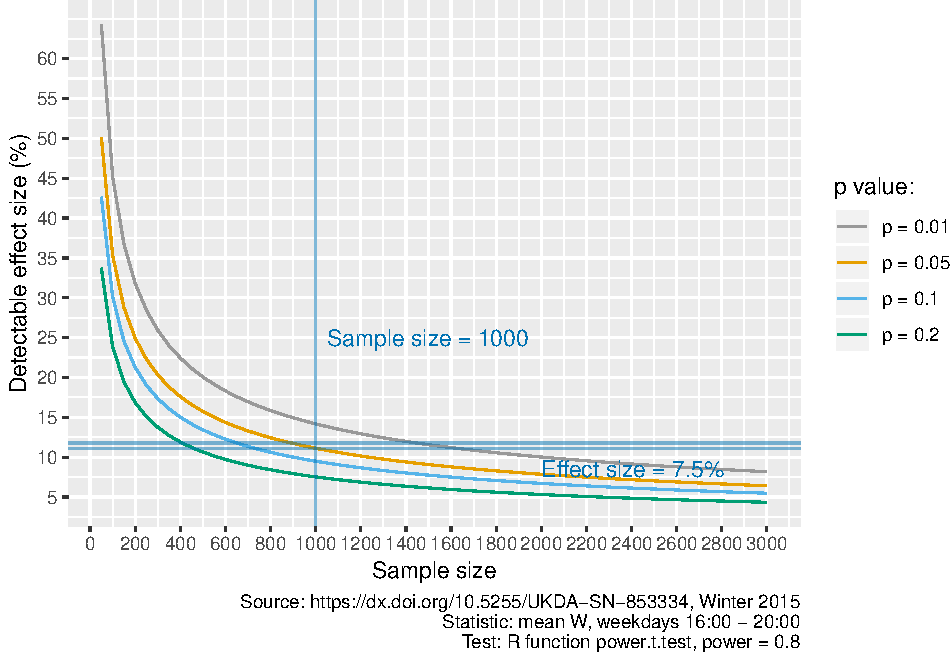
\includegraphics{sizingDemandResponseTrialsNZ_files/figure-latex/ggHPSampleSizeFig-1.pdf}

\begin{verbatim}
## Saving 6.5 x 4.5 in image
\end{verbatim}

As an illustration, \ref(fig:ggHPSampleSizeFig) shows sample size
calculations using `Heat Pump' electricity demand extracted from the
publicly available New Zealand Green Grid household electricity demand
data (Anderson et al. 2018) for winter 2014 for the peak demand period
(16:00 - 20:00) on weekdays.

As a guide, these results suggest that a trial comprising a control and
intervention sample of 1000 households (each) would be able to detect an
effect size of XXX with p = 0.05 and power = 0.8. Were a study to be
less risk averse in it's decision making then p = 0.1 may be acceptable
in which case only \textasciitilde{} XXX households would be needed in
each group (see \ref(fig:sampleSizeFig)) but the risk of a Type I error
would increase. Reducing the statistical power used would also reduce
the sample required for a given effect size tested at a given p value.
However in this case the risk of a Type II error would increase.

\section{Testing for differences: confidence intervals and p
values}\label{testing-for-differences-confidence-intervals-and-p-values}

\section{Summary and recomendations}\label{summary-and-recomendations}

\section{Runtime}\label{runtime}

Analysis completed in 51.56 seconds ( 0.86 minutes) using
\href{https://cran.r-project.org/package=knitr}{knitr} in
\href{http://www.rstudio.com}{RStudio} with R version 3.5.1 (2018-07-02)
running on x86\_64-apple-darwin15.6.0.

\section{R environment}\label{r-environment}

R packages used:

\begin{itemize}
\tightlist
\item
  base R - for the basics (R Core Team 2016)
\item
  data.table - for fast (big) data handling (Dowle et al. 2015)
\item
  lubridate - date manipulation (Grolemund and Wickham 2011)
\item
  ggplot2 - for slick graphics (Wickham 2009)
\item
  readr - for csv reading/writing (Wickham, Hester, and Francois 2016)
\item
  dplyr - for select and contains (Wickham and Francois 2016)
\item
  progress - for progress bars (Csárdi and FitzJohn 2016)
\item
  kableExtra - to create this document \& neat tables (Xie 2016)
\item
  GREENGrid - for local NZ GREEN Grid project utilities
\end{itemize}

Session info:

\begin{verbatim}
## R version 3.5.1 (2018-07-02)
## Platform: x86_64-apple-darwin15.6.0 (64-bit)
## Running under: macOS High Sierra 10.13.6
## 
## Matrix products: default
## BLAS: /Library/Frameworks/R.framework/Versions/3.5/Resources/lib/libRblas.0.dylib
## LAPACK: /Library/Frameworks/R.framework/Versions/3.5/Resources/lib/libRlapack.dylib
## 
## locale:
## [1] en_GB.UTF-8/en_GB.UTF-8/en_GB.UTF-8/C/en_GB.UTF-8/en_GB.UTF-8
## 
## attached base packages:
## [1] stats     graphics  grDevices utils     datasets  methods   base     
## 
## other attached packages:
## [1] kableExtra_0.9.0  SAVEr_0.0.1.9000  lubridate_1.7.4   readr_1.1.1      
## [5] ggplot2_3.0.0     dplyr_0.7.6       data.table_1.11.4 GREENGrid_0.1.0  
## [9] GREENGridData_1.0
## 
## loaded via a namespace (and not attached):
##  [1] Rcpp_0.12.18      lattice_0.20-35   tidyr_0.8.1      
##  [4] prettyunits_1.0.2 png_0.1-7         utf8_1.1.4       
##  [7] assertthat_0.2.0  rprojroot_1.3-2   digest_0.6.15    
## [10] R6_2.2.2          cellranger_1.1.0  plyr_1.8.4       
## [13] backports_1.1.2   evaluate_0.11     httr_1.3.1       
## [16] pillar_1.3.0      RgoogleMaps_1.4.2 rlang_0.2.2      
## [19] progress_1.2.0    lazyeval_0.2.1    readxl_1.1.0     
## [22] rstudioapi_0.7    geosphere_1.5-7   rmarkdown_1.10   
## [25] proto_1.0.0       stringr_1.3.1     munsell_0.5.0    
## [28] broom_0.5.0       compiler_3.5.1    modelr_0.1.2     
## [31] xfun_0.3          pkgconfig_2.0.2   htmltools_0.3.6  
## [34] openssl_1.0.2     tidyselect_0.2.4  tibble_1.4.2     
## [37] bookdown_0.7      fansi_0.3.0       viridisLite_0.3.0
## [40] crayon_1.3.4      withr_2.1.2       grid_3.5.1       
## [43] nlme_3.1-137      jsonlite_1.5      gtable_0.2.0     
## [46] magrittr_1.5      scales_1.0.0      cli_1.0.0        
## [49] stringi_1.2.4     mapproj_1.2.6     reshape2_1.4.3   
## [52] bindrcpp_0.2.2    sp_1.3-1          tidyverse_1.2.1  
## [55] xml2_1.2.0        rjson_0.2.20      tools_3.5.1      
## [58] forcats_0.3.0     ggmap_2.6.1       glue_1.3.0       
## [61] purrr_0.2.5       maps_3.3.0        hms_0.4.2        
## [64] jpeg_0.1-8        yaml_2.2.0        colorspace_1.3-2 
## [67] rvest_0.3.2       knitr_1.20.13     bindr_0.1.1      
## [70] haven_1.1.2
\end{verbatim}

\section*{References}\label{references}
\addcontentsline{toc}{section}{References}

\hypertarget{refs}{}
\hypertarget{ref-AECOM2011Energy}{}
AECOM. 2011. ``Energy Demand Research Project: Final Analysis.'' St
Albans: AECOM.

\hypertarget{ref-anderson_new_2018}{}
Anderson, Ben, David Eyers, Rebecca Ford, Diana Giraldo Ocampo, Rana
Peniamina, Janet Stephenson, Kiti Suomalainen, Lara Wilcocks, and
Michael Jack. 2018. ``New Zealand GREEN Grid Household Electricity
Demand Study 2014-2018,'' September.
doi:\href{https://doi.org/10.5255/UKDA-SN-853334}{10.5255/UKDA-SN-853334}.

\hypertarget{ref-CER2012Smart}{}
CER. 2012. ``Smart Meter Electricity Consumer Behaviour Trial data.''
Dublin: Irish Social Science Data Archive.
\url{http://innovation.ukpowernetworks.co.uk/innovation/en/Projects/tier-2-projects/Energywise/}.

\hypertarget{ref-progress}{}
Csárdi, Gábor, and Rich FitzJohn. 2016. \emph{Progress: Terminal
Progress Bars}. \url{https://CRAN.R-project.org/package=progress}.

\hypertarget{ref-Delmas2013Information}{}
Delmas, Magali A., Miriam Fischlein, and Omar I. Asensio. 2013.
``Information strategies and energy conservation behavior: A
meta-analysis of experimental studies from 1975 to 2012.'' \emph{Energy
Policy} 61 (October): 729--39.
doi:\href{https://doi.org/10.1016/j.enpol.2013.05.109}{10.1016/j.enpol.2013.05.109}.

\hypertarget{ref-data.table}{}
Dowle, M, A Srinivasan, T Short, S Lianoglou with contributions from R
Saporta, and E Antonyan. 2015. \emph{Data.table: Extension of
Data.frame}. \url{https://CRAN.R-project.org/package=data.table}.

\hypertarget{ref-Frederiks2016Evaluating}{}
Frederiks, Elisha R., Karen Stenner, Elizabeth V. Hobman, and Mark
Fischle. 2016. ``Evaluating energy behavior change programs using
randomized controlled trials: Best practice guidelines for
policymakers.'' \emph{Energy Research \& Social Science} 22 (December):
147--64.
doi:\href{https://doi.org/10.1016/j.erss.2016.08.020}{10.1016/j.erss.2016.08.020}.

\hypertarget{ref-Greenland2016}{}
Greenland, Sander, Stephen J. Senn, Kenneth J. Rothman, John B. Carlin,
Charles Poole, Steven N. Goodman, and Douglas G. Altman. 2016.
``Statistical Tests, P Values, Confidence Intervals, and Power: A Guide
to Misinterpretations.'' \emph{European Journal of Epidemiology} 31 (4):
337--50.
doi:\href{https://doi.org/10.1007/s10654-016-0149-3}{10.1007/s10654-016-0149-3}.

\hypertarget{ref-lubridate}{}
Grolemund, Garrett, and Hadley Wickham. 2011. ``Dates and Times Made
Easy with lubridate.'' \emph{Journal of Statistical Software} 40 (3):
1--25. \url{http://www.jstatsoft.org/v40/i03/}.

\hypertarget{ref-RockyMountainInstitute2006Automated}{}
Institute, Rocky Mountain. 2006. ``Automated demand response system
pilot: Final report.''
\url{https://www.smartgrid.gov/files/Aumated_Demd_Response_System_Pilot_Volume_1_Intro_Exec_Summa.pdf}.

\hypertarget{ref-baseR}{}
R Core Team. 2016. \emph{R: A Language and Environment for Statistical
Computing}. Vienna, Austria: R Foundation for Statistical Computing.
\url{https://www.R-project.org/}.

\hypertarget{ref-Schofield2015Experimental}{}
Schofield, James, Richard Carmichael, Simon Tindemans, Matt Woolf, Mark
Bilton, and Goran Strbac. 2015. ``Experimental validation of residential
consumer responsiveness to dynamic time-of-use pricing.'' In \emph{23
International Conference on Electricity Distribution}.

\hypertarget{ref-Srivastava2018Assessing}{}
Srivastava, Aman, Steven Van Passel, and Erik Laes. 2018. ``Assessing
the Success of Electricity Demand Response Programs: A Meta-Analysis.''
\emph{Energy Research \& Social Science} 40 (June): 110--17.
doi:\href{https://doi.org/10.1016/j.erss.2017.12.005}{10.1016/j.erss.2017.12.005}.

\hypertarget{ref-energyWiseT1}{}
UKPN. 2017. ``The Final Energy Saving Trial Report.'' London: UK Power
Networks.
\url{http://innovation.ukpowernetworks.co.uk/innovation/en/Projects/tier-2-projects/Energywise/}.

\hypertarget{ref-energyWiseT2}{}
---------. 2018. ``The Energy Shifting Trial Report.'' London: UK Power
Networks.
\url{http://innovation.ukpowernetworks.co.uk/innovation/en/Projects/tier-2-projects/Energywise/}.

\hypertarget{ref-wasserstein2016}{}
Wasserstein, Ronald L., and Nicole A. Lazar. 2016. ``The Asa's Statement
on P-Values: Context, Process, and Purpose.'' \emph{The American
Statistician} 70 (2). Taylor \& Francis: 129--33.
doi:\href{https://doi.org/10.1080/00031305.2016.1154108}{10.1080/00031305.2016.1154108}.

\hypertarget{ref-ggplot2}{}
Wickham, Hadley. 2009. \emph{Ggplot2: Elegant Graphics for Data
Analysis}. Springer-Verlag New York. \url{http://ggplot2.org}.

\hypertarget{ref-dplyr}{}
Wickham, Hadley, and Romain Francois. 2016. \emph{Dplyr: A Grammar of
Data Manipulation}. \url{https://CRAN.R-project.org/package=dplyr}.

\hypertarget{ref-readr}{}
Wickham, Hadley, Jim Hester, and Romain Francois. 2016. \emph{Readr:
Read Tabular Data}. \url{https://CRAN.R-project.org/package=readr}.

\hypertarget{ref-knitr}{}
Xie, Yihui. 2016. \emph{Knitr: A General-Purpose Package for Dynamic
Report Generation in R}. \url{https://CRAN.R-project.org/package=knitr}.


\end{document}
